\section{Background}
\label{sec:background}
Static analysis is a technique for automatically analyzing the behavior of software
without executing it. It has a wide range of applications, including code optimization,
bug detection, security vulnerability analysis, and program understanding.
In this chapter, we will focus on two specific types of static analysis:
control-flow analysis and dataflow analysis.

Control-flow analysis involves analyzing the control flow of a program,
which refers to the order in which the statements in the program are executed.
This type of analysis is useful for understanding the logical structure of a
program and identifying potential errors, such as uninitialized variables or
infinite loops.

Dataflow analysis, on the other hand, involves analyzing the flow of data through
a program. This includes tracking the sources and uses of variables, as well as
determining the possible values that variables can take on at different points in
the program. Dataflow analysis can be used to optimize code, detect defects, and
perform other tasks such as type checking.

Both control-flow analysis and dataflow analysis are important tools for improving
the quality and reliability of software. In the following sections, we will delve
deeper into each of these techniques and discuss their applications and limitations.



\subsection{Control-flow analysis}

Control-flow analysis involves analysing the control flow of the program, which refers
to the execution order of the program's statements. It aids in comprehending the logical
structure of a program and recognising potential flaws, such as uninitialized variables
and infinite loops.
Control-flow analysis is the basis for many other static analyses including dataflow analysis.


Control-flow analysis can be performed without executing the program, which makes
it a useful analysis for debugging and testing. In addition, control-flow analysis
can provide valuable insights into the structure and behavior of a program,
which can help with program understanding and maintenance.
However, one major limitation of control-flow analysis is that it is subject to the Rice-Turing theorem result,
meaning that it is not always possible to determine the exact control flow of a program.
Additionally, control-flow analysis may not be sound or complete, or may not
strive for either property. This means that it may not always accurately capture
the full behavior of a program, particularly in cases involving complex
interactions or data-dependent behavior.

There are two main approaches to constructing the control-flow graph for a program:
on the source-level and on the intermediate representation. The source-level approach
involves analyzing the source code of a program and constructing the control-flow graph
directly from the source code. The intermediate representation approach involves
first converting the source code into an intermediate representation, such as bytecode,
and then constructing the control-flow graph from the intermediate representation.

Constructing the control-flow graph (CFG) on the source level has several advantages.
One of the main benefits is that it allows for the analysis to be performed directly
on the source code of the program, which can be more easily understood by humans.
This can be particularly useful for debugging and program understanding tasks,
as it allows the analysis to be performed in the context of the original program.

Another advantage of constructing the CFG on the source level is that it does not
require the generation of an intermediate representation (IR). This can make the
analysis faster and more efficient, as it avoids the overhead of IR generation.
In addition, constructing the CFG on the source level can work with semantically
and syntactically broken code, which can be useful for analyzing programs with
errors or inconsistencies.
Furthermore, in situations where the (IR) must be generated in real-time,
such as for integrated development environment (IDE) analysis integration and support,
the overhead of code generation and optimization may make this process too expensive.
In such cases, constructing the control-flow graph (CFG) on the source level
may be a more efficient option.

However, there are also some disadvantages to constructing the CFG on the source level.
One of the main limitations is that it can be more difficult to accurately capture the
control-flow of a program when working with the source code. This is because the source
code may contain various constructs, such as macros and preprocessor directives, that
can complicate the analysis. In addition, the source code may be written in a variety
of languages with different syntax and semantics, which can make it challenging to
design a single analysis that works across all languages.

\begin{figure}[h]
  \centering
\begin{tabular}{l r}
  \begin{lstlisting}[language=JastAdd]
void foo(){
  int x = 0;
  if (x > 0) {
    x = 1;
  } else {
    x = -1;
  }
}
  \end{lstlisting} &\hspace{2.5cm}
  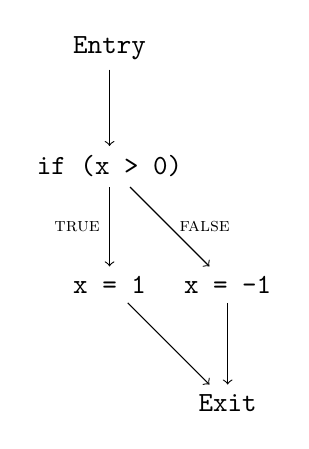
\begin{tikzpicture}[node distance=1.5cm, baseline=(current bounding box.center)]
      \node (start) [rectangle] {\texttt{Entry}};
      \node (if) [rectangle, below of=start] {\texttt{if (x > 0)}};
      \node (then) [rectangle, below of=if] {\texttt{x = 1}};
      \node (else) [rectangle, right of=then] {\texttt{x = -1}};
      \node (end) [rectangle, below of=else] {\texttt{Exit}};
      \draw [->] (start) -- (if);
      \draw [->] (if) -- node [left, font=\scriptsize] {\textsc{true}} (then);
      \draw [->] (if) -- node [right,  font=\scriptsize]{\textsc{false}} (else);
      \draw [->] (then) -- (end);
      \draw [->] (else) -- (end);
  \end{tikzpicture}
  \end{tabular}
  \caption{\label{fig:cfgsourcelevel}Source level control-flow graph of the \texttt{foo} method, showing the branching behavior of the if statement.}
\end{figure}


\begin{figure}[h]
  \centering
\begin{tabular}{l r}

\begin{lstlisting}[language=bytecode, frame=none]
0 : iconst_0
1 : istore_1
2 : iload_1
3 : ifle        10
6 : iconst_1
7 : istore_1
8 : goto        13
11: iconst_m1
12: istore_1
13: return
\end{lstlisting}
&\hspace{2.5cm}
\begin{tikzpicture}[
  node distance=0.4cm,
  every node/.style={shape=rectangle, align=center},
  baseline=(current bounding box.center)]
  % Nodes
  \node (0) {0};
  \node (1) [below=of 0] {1};
  \node (2) [below=of 1] {2};
  \node (3) [below=of 2] {3};
  \node (6) [left=of 3] {6};
  \node (7) [below=of 6] {7};
  \node (8) [below=of 7] {8};
  \node (11) [right=of 3] {11};
  \node (12) [below=of 11] {12};
  \node (14) [below=of 3] {};
  \node (15) [below=of 14] {};
  \node (13) [below=of 15] {13};
  
  % Edges
  \path[->] (0) edge (1) (1) edge (2) (2) edge (3) (3) edge[bend right] (6) (3) edge[bend left] (11) (6) edge (7) (7) edge (8) (8) edge (13) (11) edge (12) (12) edge (13);
  
  \draw[dashed] (1.north west) rectangle (2.south east);
  \draw[dashed] (6.north west) rectangle (8.south east);
  \draw[dashed] (11.north west) rectangle (12.south east);

\end{tikzpicture}
\end{tabular}
\caption{\label{fig:cfgintermediatelevel}Bytecode control-flow graph of the \texttt{foo} method. Each dashed box represents a basic block.}
\end{figure}


The examples in Figures~\ref{fig:cfgsourcelevel} and~\ref{fig:cfgintermediatelevel} show the control-flow 
graphs of the simple \texttt{foo} method.


\subsection{Dataflow Analysis}
\label{sec:dataflowanalysis}
Dataflow analysis is a technique used in computer science to analyze the flow of 
data through a program. It has its roots in the field of program optimization, 
where it was originally used to identify opportunities for improving the performance 
of programs by removing unnecessary computations e.g., Very Busy Expression or Available Expression analyses~\cite{aho2007compilers,vallee-rai10soot,falconer2007deepweaver,sagiv1996ide,kildall1973dataflow}.
Dataflow analysis involves tracking the flow of data through a program by 
identifying the variables that are defined and used at each point in the program's 
control flow. This information can be used to optimize the program by eliminating 
unnecessary computations and improving the use of available resources.
One of the primary advantages of dataflow analysis is its ability to handle programs 
with complex control flow, such as those with loops and conditional statements. 

In the context of bug detection~\cite{spoon, fink2012wala}, dataflow analysis can be used to identify 
potential sources of errors in a program by tracking the flow of data through 
the program and identifying points where data may be used in unexpected or 
incorrect ways. This can be particularly useful in identifying bugs that may 
not be immediately apparent, such as those that only occur under certain 
conditions or when certain combinations of input data are used.
Many tools for static analysis of Java programs, such as FindBugs~\cite{findbugs},
SpotBugs~\cite{spotbugs}, and PMD~\cite{copeland2005pmd}, use dataflow analysis to identify
potential bugs in Java programs. 
% I looked here how they cited pmd, findbugs and spotbugs. https://ieeexplore.ieee.org/stamp/stamp.jsp?tp=&arnumber=8103456

Dataflow analysis can also be used to identify potential security vulnerabilities 
in software~\cite{flowDroid,piskachev2021secucheck,lawall10coccinelle}. By tracking the flow of sensitive data through a program and  
identifying points where it may be exposed to unauthorized access or manipulation, 
dataflow analysis can help to identify potential vulnerabilities that could be 
exploited by attackers. 

